\documentclass[10pt,oneside]{article}
\usepackage[T1]{fontenc}
\usepackage[utf8]{inputenc}
%\DeclareUnicodeCharacter{00A0}{ }
\usepackage[adobe-utopia]{mathdesign}

\usepackage{amsmath}
\usepackage[francais]{babel}
\usepackage[dvips]{graphicx}
%\usepackage{here}
\usepackage{framed}
\usepackage[normalem]{ulem}
\usepackage{fancyhdr}
\usepackage{titlesec}
\usepackage{vmargin}

\usepackage{amsmath}
\usepackage{ifthen}
\usepackage{multirow}
\usepackage{multicol} % Portions de texte en colonnes

%\usepackage{xltxtra} % Logo XeLaTeX
%\usepackage{pst-solides3d}
\usepackage{color}
%\usepackage{colortbl}
\usepackage{titletoc} % Pour la mise en forme de la table des matières

%\usepackage[crop=off]{auto-pst-pdf}
%\usepackage{bclogo}


%\usepackage{longtable}
%\usepackage{flafter}%floatants après la référence
%\usepackage{pst-solides3d}
%\usepackage{pstricks}
%\usepackage{minitoc}
%\setcounter{minitocdepth}{4}
%\usepackage{draftcopy}% "Brouillon"
%\usepackage{floatflt}
%\usepackage{psfrag}
%\usepackage{listings} % Permet d'insérer du code de programmation
%\usepackage{lmodern}
%\usepackage[adobe-utopia,uppercase=upright,greeklowercase=upright]{mathdesign}
%\usepackage{minionpro}
%\usepackage{pifont}
%\usepackage{amssymb}
%\usepackage[francais]{varioref}

\setmarginsrb{1.5cm}{1cm}{1cm}{1.5cm}{1cm}{1cm}{1cm}{1cm}

\definecolor{gris25}{gray}{0.75}
\definecolor{bleu}{RGB}{18,33,98}
\definecolor{bleuf}{RGB}{42,94,171}
\definecolor{bleuc}{RGB}{231,239,247}
\definecolor{rougef}{RGB}{185,18,27}
\definecolor{rougec}{RGB}{255,230,231}
\definecolor{vertf}{RGB}{103,126,82}
\definecolor{vertc}{RGB}{220,255,191}
\definecolor{violetf}{RGB}{112,48,160}
\definecolor{violetc}{RGB}{230,224,236}
\definecolor{jaunec}{RGB}{220,255,191}

\usepackage[%
    pdftitle={SLCI - DS3},
    pdfauthor={Xavier Pessoles},
    colorlinks=true,
    linkcolor=blue,
    citecolor=magenta]{hyperref}



% \makeatletter \let\ps@plain\ps@empty \makeatother
%% DEBUT DU DOCUMENT
%% =================
\sloppy
\hyphenpenalty 10000

\newcommand{\Pointilles}[1][3]{%
\multido{}{#1}{\makebox[\linewidth]{\dotfill}\\[\parskip]
}}

\begin{document}


\newboolean{prof}
\setboolean{prof}{false}
%------------- En tetes et Pieds de Pages ------------
\pagestyle{fancy}
\renewcommand{\headrulewidth}{0.2pt}

\fancyhead{}
\fancyhead[L]{PTSI -- Sciences Industrielles pour l'Ingénieur}
\fancyhead[R]{Lycée Jules Haag -- Besançon}


\renewcommand{\footrulewidth}{0.2pt}
\fancyfoot[C]{\bfseries \thepage}
\fancyfoot[L]{2010 -- 2011}
\ifthenelse{\boolean{prof}}{%
\fancyfoot[R]{DS 3 -- SLCI}
}{%
\fancyfoot[R]{DS 3 -- SLCI}
}

%\fancyfoot[RO]{Version du \today}
% \fancyfoot[LE]{Version du \today}
% \fancyfoot[RO]{\textcolor{gris25}{Version rapporteurs}}
% \fancyfoot[LE]{\textcolor{gris25}{Version rapporteurs}}
% \fancyfoot[R]{\textcolor{gris25}{Version rapporteurs}}
% ----------------------------------------------------



\vspace{1cm}

\begin{center}
 \huge\textsc{Devoir Surveille 3}

\vspace{1cm}

 \large\textsc{Vendredi 12 novembre 2010 -- 4 heures}
\end{center}

\vspace{1cm}


\noindent\rule{\linewidth}{.2pt}
\begin{center}
 \large\textbf{CI : 1} \textit{AF : Fonctionnalités, architecture et structure des systèmes pluri techniques}

 \large\textbf{CI : 5} \textit{Communication technique : schémas et géométrie des pièces}

 \large\textbf{CI : 7} \textit{SLCI : Comportement et modélisation des systèmes automatiques. Identification }

 \large\textbf{CI : 8} \textit{Seq : Commande et comportement des systèmes à événements discrets (Combinatoire et Séquentiel)}
\end{center}
\noindent\rule{\linewidth}{.2pt}


\vfill

\textbf{Contenu du sujet :}
\begin{itemize}
\item \textbf{Partie 1 : Système de convoyage et d'élévation -- 1 heure }
\item \textbf{Partie 2 : Dessin industriel -- 1 heure }
\item \textbf{Partie 3 : Système de freinage de l'Airbus A318 -- 2 heures}
\end{itemize}

\vfill

\textbf{Consignes et recommandations :}
\begin{itemize}
\item \textbf{Il est recommandé de lire le sujet dans son intégralité avant de
répondre aux questions}
\item \textbf{Les question sont numérotées et ordonnées mais beaucoup d'entre elles sont indépendantes.}
\item \textbf{Il est recommandé de passer une heure sur les parties 1 heure sur la partie 1, une heure sur la partie 2, 2 heures sur la partie 3}
\item \textbf{Les parties seront notées proportionnellement aux temps proposés ci-dessus.}
\item \textbf{Les réponses sont à donner sur feuille pour la partie 3. Pour cette partie il est particulièrement recommandé de :}
\begin{itemize}
\item \textit{rappeler, sur sa copie le numéro de la question avant de développer sa réponse;}
\item \textit{de bien respecter l'ensemble des notations alphabétiques et numériques définies dans le sujet et de préciser ses propres notations lorsque cela s'avère nécessaire;}
\item \textit{de justifier ses hypothèses, et de rédiger clairement ses réponses.}
\item de rendre les documents réponse.

\end{itemize}
\end{itemize}

\vfill

\begin{center}
\textsc{\textbf{Tout Document Interdit}}

 \textsc{\textbf{Calculatrices, Téléphones Portables, Lecteur MP3 ...
Interdits}}
\end{center}

\newpage

\noindent\rule{\linewidth}{.2pt}
\begin{center}
 \LARGE\textbf{\textsc{
Système de freinage de l'Airbus A318
}}
\end{center}
\noindent\rule{\linewidth}{.2pt}

\section{Présentation du système}
\begin{center}
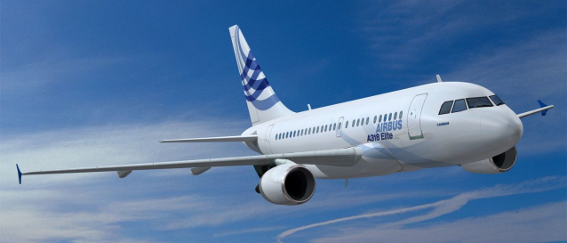
\includegraphics[width=.8\textwidth]{png/image1.png}

\textbf{Figure 1 :} Airbus A318
\end{center}

Le freinage est une des fonctions vitales d’un avion, au même titre que la
propulsion ou la sustentation.
C’est grâce à lui que l’avion peut s’immobiliser après l’atterrissage, circuler
au sol en toute sécurité mais
également s’arrêter en cas d’urgence lors d’une interruption de décollage alors
que l’avion est à pleine
charge de carburant et lancé à la vitesse de décollage (même si le risque est de
l’ordre de 1 pour 1 million
de décollages). Outre les freins, le pilote peut aussi actionner les inverseurs
de poussée des moteurs et les
aérofreins.
On s'intéresse au système de freinage des roues de l’Airbus A318, avion
commercial de 120 places et de
rayon d’action de 3240 km. La vitesse de décollage est estimée à 240 km/h. Pour
les atterrisseurs, on
distingue (voir figure 2) :
\begin{itemize}
 \item  le train avant qui, en dehors de
        l’appui, est orientable ce qui lui
        permet d’agir sur les trajectoires
        au sol mais qui n’est pas équipé
        de freins;
\item les deux trains principaux au
        niveau des ailes, chacun portant
        deux roues freinées
        indépendamment. 
\end{itemize}


\subsection*{Description du système de freinage}

    Il existe deux modes de commande du système de freinage :
\begin{itemize}
 \item le \textbf{mode normal} (Normal Braking) contrôlé par un ordinateur
dénommé BSCU
(Braking/Steering
         Control Unit). Le BSCU contrôle les servovalves (une par roue) qui
alimentent les pistons
         presseurs. Ces pistons exercent alors une action sur les roues qui
diminue alors la vitesse de
         l'avion. La pression hydraulique est fournie par le groupe hydraulique
principal;
\item le \textbf{mode alternatif} (Alternate braking) contrôlé par un ordinateur
dénommé
ABCU (Alternate
         Braking Control Unit). Ce mode prend automatiquement la relève du mode
normal s’il y a
         dysfonctionnement de ce dernier ou si le contrôle anti-dérapage
(Anti-Skid) de l’avion est
         supprimé. En mode alternatif, la pression hydraulique est fournie par
un groupe hydraulique
         secondaire.
\end{itemize}

En mode normal, il est possible de commander le freinage de deux façons
différentes :
\begin{itemize}
 \item soit \textbf{manuellement} par appui sur les pédales de frein (voir
figure 3) : pour chaque pilote, les
         pédales gauche et droite sont indépendantes. L’appui sur la pédale
gauche agit sur le freinage des
         roues du train principal gauche, l’appui sur celle de droite agit sur
le freinage des roues du train
         principal droit. Les unités de transmission (Brake Pedal Transmitter
Unit) situées sous les pédales
         émettent des signaux électriques vers le BSCU ou vers l’ABCU
proportionnels à la course des
         pédales de frein;
\item soit \textbf{automatiquement} suivant trois modes de décélération : LO,
MED, MAX. La sélection se fait
         à partir de trois boutons situés sur le tableau de bord (voir figure
4). Le mode manuel est rétabli si
         le pilote, en appuyant sur les pédales de frein, génère une consigne de
décélération $a_p$ supérieure à
         la consigne de décélération $a_c$ du mode automatique sélectionné.
\end{itemize}                                                    


\begin{center}
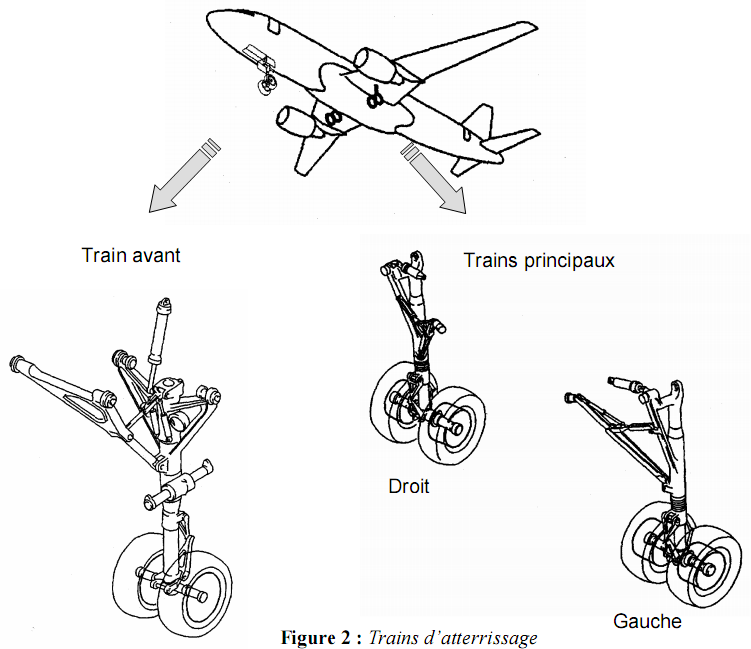
\includegraphics[width=.6\textwidth]{png/image2.png}

\textbf{Figure 2 :} Train d'atterrissage
\end{center}

\begin{center}
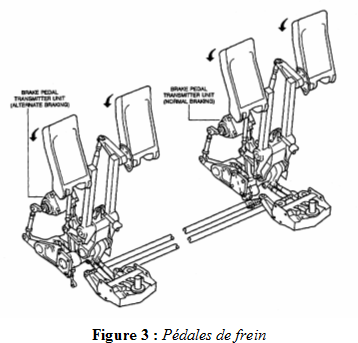
\includegraphics[width=.5\textwidth]{png/image3.png}
\end{center}
   
\begin{center}
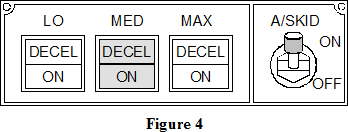
\includegraphics[width=.4\textwidth]{png/image4.png}
\end{center}            

Les modes LO et MED sont utilisés lors de l’atterrissage. Ils correspondent
respectivement à une
décélération de l’avion de $-1,7 ms^{-2}$ et de $-3 ms^{-2}$. Le mode MAX est
exclusivement sélectionné lors du
décollage, en cas d’interruption de ce dernier. Il correspond à une décélération
théorique de $-10 ms^{-2}$
supérieure à la décélération maximale de l’avion.

En mode normal (manuel ou automatique), le BSCU contrôle l’anti-dérapage (Anti
Skid) de chaque roue
tant que la vitesse de l’avion est supérieure à $5\;m/s$.
En mode alternatif, seule la commande manuelle est disponible avec ou sans
anti-dérapage.
 

\section{Description fonctionnelle du système de freinage}

On donne ci-dessous le SADT de niveau A-0 qui décrit la fonction principale du système de freinage.

\begin{center}
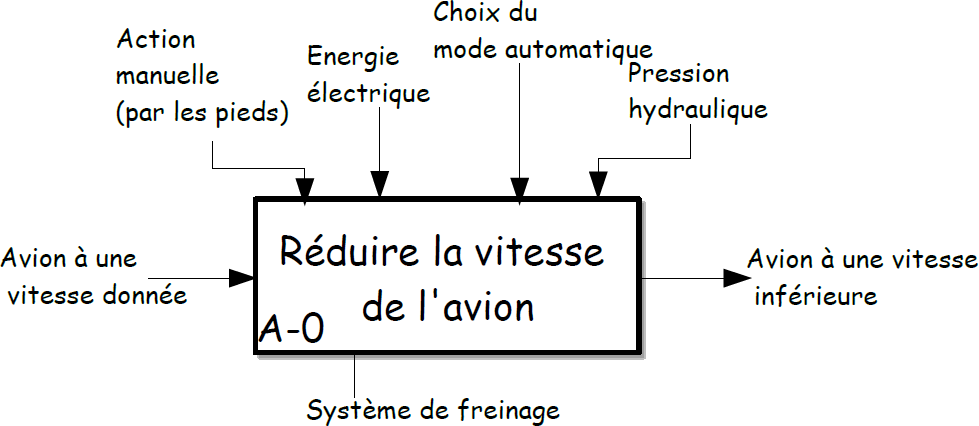
\includegraphics[width=.5\textwidth]{png/image5.png}
\end{center}

\paragraph{}
\textit{Compléter à partir des explications précédentes et du SADT A-0, le SADT de niveau A0.}

On s'intéresse dans toute la suite du sujet uniquement au mode de décélération automatique du mode
normal, qui consiste à asservir en décélération le freinage de l'avion.
Bien que les variables manipulées par le BSCU soient des variables numériques, on les considèrera, par la
suite, comme étant analogiques. Le système est donc, sur le plan théorique, supposé linéaire, continu et
invariant.

L'utilisateur donne une consigne numérique $a_c(t)$ qui est comparée à la valeur numérique $a_m(t)$
fournie par l'accéléromètre, image de la décélération réelle $a(t)$. Le BSCU génère à partir de cet écart
$\varepsilon(t)$ , une commande $i(t)$ pour la servovalve. Celle-ci fournit alors la pression $p_h(t)$ aux freins qui
entraîne alors la décélération $a(t)$ de l'avion.

\paragraph{}
\textit{Réaliser un schéma-bloc fonctionnel de l'asservissement en décélération à partir des
indications ci-dessus. On prendra $a_c(t)$ comme entrée et $a(t)$ comme sortie.}

\section{Modélisation du système de freinage}
Dans cette seconde partie, on souhaite définir un modèle pour l'asservissement en décélération. Pour cela,
on propose de déterminer une fonction de transfert pour tous les constituants.

\subsection{Modélisation de la servovalve}

Une servovalve électrohydraulique est un appareil qui convertit une grandeur électrique (courant ou
tension) en une grandeur hydraulique proportionnelle (débit ou pression).
La servovalve la plus utilisée est la servovalve en débit ou pression à 2 étages. Elle est constituée de trois
éléments :
\begin{itemize}
\item un actionneur de type moteur électrique ;
\item un amplificateur hydraulique constitué d’un mécanisme buse-palette ;
\item un tiroir de distribution.
\end{itemize}

\begin{center}
\begin{tabular}{cc}
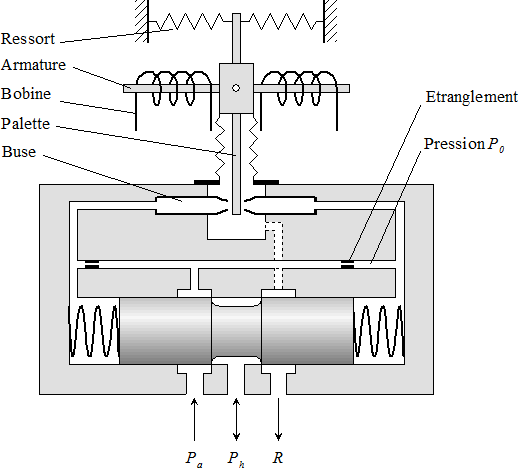
\includegraphics[width=.45\textwidth]{png/image6.png}&
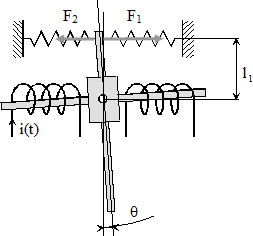
\includegraphics[width=.45\textwidth]{png/image7.png}
\end{tabular}
\end{center}

L’armature du moteur à courant continu se prolonge dans l’entrefer d’un circuit magnétique. Le passage
d’un courant continu dans les deux bobines situées de part et d’autre de l’armature provoque le
basculement de cette dernière d’un angle $\theta$.

L’armature est solidaire d’une palette plongeant dans l’amplificateur hydraulique et dont l’extrémité est
située entre deux buses. Le mouvement de rotation de l’ensemble armature-palette vient étrangler le débit
fluide traversant l’une ou l’autre des buses. La pression différentielle ainsi créée se répercute aux deux
extrémités du tiroir du distributeur et provoque son déplacement.

Ce tiroir possède trois orifices de contrôle, $P_a$ (Alimentation), $P_h$ (Utilisation), $R$ (Retour à la bâche). La pression $P_h$ est proportionnelle au déplacement du tiroir compté à partir de la position zéro (position du
milieu).

A titre indicatif, le diamètre $d$ des buses est de l’ordre de quelques dixièmes de millimètres et l’écart $e$
entre la buse et la palette de l’ordre de quelques centièmes de millimètres.

On donne ci-dessous la caractéristique reliant l'intensité $i(t)$ du moteur à l'angle $\theta(t)$ dont bascule
l'armature.

\begin{center}
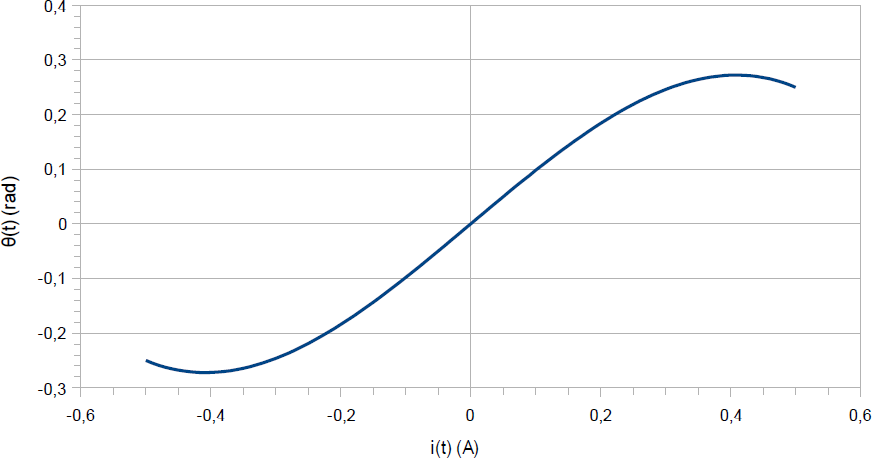
\includegraphics[width=.8\textwidth]{png/image8.png}
\end{center}

\paragraph{}
\textit{Que peut-on dire de cette caractéristique sur tout le domaine de variation de $i(t)$ ? Sachant
que $\theta$ est très petit (varie autour de 0), on utilise la relation suivante $\theta(t)=K_1i(t)$.
 Déterminer la valeur de $K_1$ à partir de la courbe.}

On admet que, pour le système buse-palette, la rotation d'angle $\theta$ de la palette se traduit par un
accroissement ou diminution de la distance buse-palette. Les sections de fuite sont alors augmentées ou
diminuées, ce qui entraîne une augmentation ou diminution des pressions $P_A$ et $P_B$ proportionnelle à
$\Delta S$.

\begin{center}
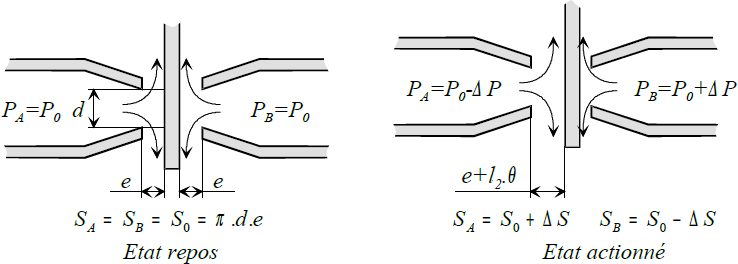
\includegraphics[width=.8\textwidth]{png/image9.png}
\end{center}

On peut alors définir les relations suivantes :
$$\Delta S=K_2 \theta$$
$$\Delta P=K_3 \Delta S$$
Cette pression différentielle permet de mettre en mouvement le tiroir de la servovalve.

En situation repos, lorsque $P_A=P_B=P_0$, le tiroir est en position milieu, $z = 0$ ( cf figure ci-dessous).

\begin{center}
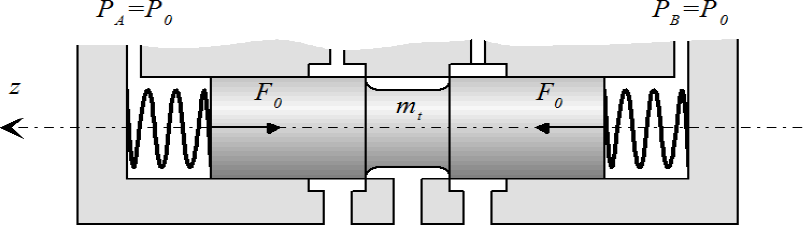
\includegraphics[width=.5\textwidth]{png/image10.png}

\textit{Tiroir en position repos}
\end{center}

En position travail, la pression différentielle se répercute aux extrémités du tiroir et provoque son
déplacement.

\begin{center}
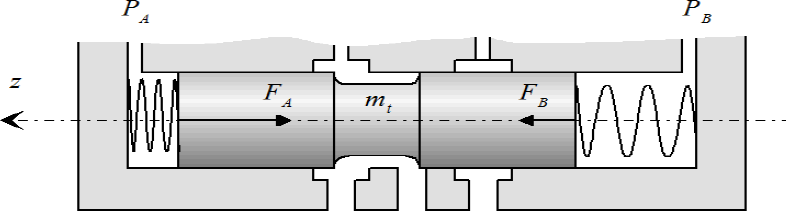
\includegraphics[width=.5\textwidth]{png/image11.png}

\textit{Tiroir en position travail}
\end{center}

On utilise les notations suivantes :
\begin{itemize}
\item $m_t$ : masse du tiroir ;
\item $S_t$ : section du tiroir à ses extrémités ;
\item $F_A$ et $F_B$ : efforts exercés par les deux ressorts de coefficient de raideur $k_t$ montés de part et d’autre
du tiroir du distributeur ;
\item $c_t$ : coefficient de frottement visqueux entre tiroir et cylindre.
\end{itemize}

Le principe fondamental de la dynamique appliqué au tiroir donne la relation suivante :
$$
m_t\dfrac{d^2z(t)}{dt^2} = -2k_tz(t) + 2S_t\Delta P(t) -c_t \dfrac{dz(t)}{dt}
$$

\paragraph{}
\textit{Calculer la fonction de transfert $H_t(p)=\dfrac{Z(p)}{\Delta P(p)}$ 
où $Z(p)$ et $\Delta P(p)$ sont les transformées de Laplace de $z(t)$ et 
$\Delta P(t)$ en précisant l'hypothèse retenue.}

\paragraph{}
\textit{Mettre cette fonction de transfert sous forme canonique et donner son ordre.}

On admet pour finir que la pression d'utilisation $P_h(t)$ du fluide est proportionnelle au déplacement $z(t)$
du tiroir : $P_h(t)=K_4 z(t)$.

\paragraph{}
\textit{\`A partir de toutes les informations précédentes (modélisation armature, buse/palette,
tiroir...), compléter le schéma-bloc de la servovalve donné dans le document réponse, en précisant les
fonctions de transfert de chaque bloc (utiliser les notations algébriques).}

\paragraph{}
\textit{En déduire la fonction de transfert $S_v(p)=\dfrac{P_h(p)}{I(p)}$ de la servovalve.}

\paragraph{}
\textit{Montrer qu'elle peut se mettre sous la forme d'un système du second ordre :}
$$
S_v(p)=\dfrac{P_h(p)}{I(p)}=\dfrac{K_{sv}}{1+\dfrac{2\xi p}{\omega_0}+\dfrac{p^2}{\omega_0^2}}
$$
\textit{où on donnera les expressions littérales de $K_{sv}$, $\xi$ et $\omega_0$.}

On souhaite que la réponse à une entrée $i(t)$ de type échelon de valeur $i_0$ soit la plus rapide possible \textbf{sans toutefois produire de dépassement.}

\paragraph{}
\textit{A quelle valeur de $\xi$ correspond cette spécification ?}

\paragraph{}
\textit{Démontrer que cette condition ne peut être satisfaite que si $k_t=\dfrac{c_t^2}{8m_t}$.}

\paragraph{}
\textit{Montrer alors que la fonction de transfert de la servovalve peut se mettre sous la forme :}
$$
S_v(p)=\dfrac{P_h (p)}{I(p)}=\dfrac{K_{sv}}{\left( 1+T_{sv} p\right)^2 }
$$
\textit{on donnera l'expression littérale de $T_{sv}$.}

\paragraph{}
\textit{Déterminer la réponse indicielle $P_h(t)$ pour une entrée échelon de valeur $i(t)=i_0 u(t)$.}

On rappelle que $\mathcal{L}\left(te^{-at}u(t)\right)=\dfrac{1}{\left(p+a\right)^2}$.

\paragraph{}
\textit{Vous l'attendiez, la voilà, voici la question cachée. En hommage au professeur de mathématique, voici la question : 
Logarithme et Exponentielle sont dans un café, qui paie l'addition ?}
\subsection{Modélisation de l'accéléromètre}
La centrale inertielle contient des accéléromètres qui permettent de mesurer les accélérations suivant les
trois directions $x_a$, $y_a$, $z_a$ d’un repère lié à l’avion.

L’accéléromètre renvoie au BSCU un signal électrique $u_a(t)$ image de l’accélération $a(t)$ suivant la
direction $x_a$. La tension $u_a(t)$ est convertie en grandeur numérique $a_m$ par un convertisseur analogique-numérique
et rangée dans la mémoire du BSCU.

\subsection*{Principe de l’accéléromètre}
Un accéléromètre (voir figure ci-dessous) est constitué de deux solides
$S_1$ et $S_2$ :
\begin{itemize}
\item $S_1$, le corps, est lié à l’avion,
\item $S_2$ est lié à $S_1$ par l’intermédiaire d’un ressort de raideur $k_a$ et d’un frottement visqueux de valeur $c_a$.
\end{itemize}

\begin{center}
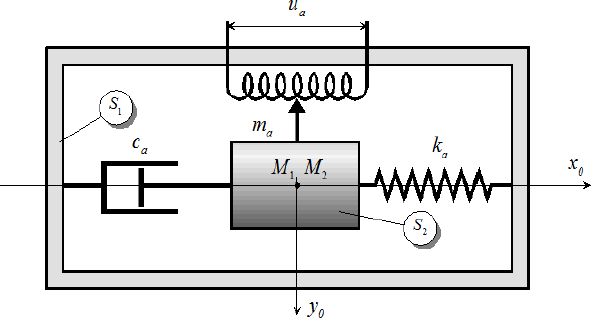
\includegraphics[width=.5\textwidth]{png/image12.png}

\textit{Accéléromètre en position repos}
\end{center}

On considère (voir figure ci-dessus) deux points $M_1$ et $M_2$ appartenant respectivement à $S_1$ et $S_2$. On note
$x_1(t)$ et $x_2(t)$ leurs coordonnées dans un repère 
$\left(O,\overrightarrow{x_0},\overrightarrow{y_0},\overrightarrow{z_0}\right)$.

On considère nulles les conditions initiales. En particulier, à l’état repos, $M_1$ et $M_2$ sont confondus.
Quand $S_1$ est animé d’un mouvement de translation suivant $x_0$, on note :
\begin{equation}
\varepsilon(t)=x_1(t)-x_2(t)
\end{equation}

\begin{equation}
a(t)=\dfrac{d^2x_1(t)}{dt^2} \text{ accélaration de } S_1
\end{equation}


\begin{center}
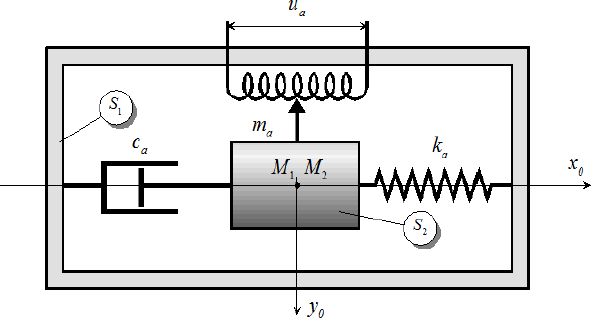
\includegraphics[width=.5\textwidth]{png/image12.png}

\textit{Accéléromètre en action}
\end{center}

D’autre part, par application du principe fondamental de la dynamique, on a :

\begin{equation}
m_a\dfrac{d^2x_2(t)}{dt^2}=c_a\left( \dfrac{dx_1(t)}{dt} - \dfrac{dx_2(t)}{dt}\right)
+k_a\left( x_1(t)-x_2(t)\right) \quad \mathrm{avec} \quad m_a, c_a, k_a \quad \mathrm{constantes}
\end{equation}

Le solide $S_2$ est relié à un potentiomètre qui renvoie une tension $u_a$ proportionnelle au déplacement $\varepsilon$ du solide $S_2$ par rapport à $S_1$. On note : 

\begin{equation}
u_a(t)=K_p \varepsilon(t)
\end{equation}

Finalement, le CAN (convertisseur analogique numérique) fournit la valeur $a_m$ telle que :
\begin{equation}
a_m(t) = K_{CAN} u_a (t) 
\end{equation}

\paragraph{}
\textit{Déterminer les transformées de Laplace des expressions (1) à (5).}

\paragraph{}
\textit{En déduire les transmittances $G_i$ du schéma bloc ci-après.}

\begin{center}
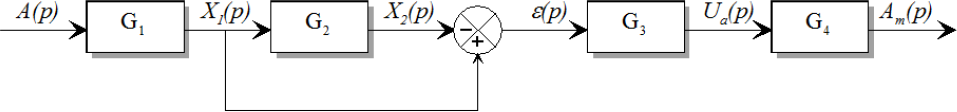
\includegraphics[width=.8\textwidth]{png/image14.png}
\end{center}

\paragraph{}
\textit{En déduire la fonction de transfert $\dfrac{A_m(p)}{A(p)}$ et montrer quelle peut se mettre sous la
forme :}
$$
\dfrac{A_m(p)}{A(p)} = \dfrac{K_{acc}}{1+2\dfrac{\xi_a p}{\omega_a} + \dfrac{p^2}{\omega_a^2}}
$$
\textit{Donner les expressions de $K_{acc}$, $\xi_a$ et $\omega_a$.}

\paragraph{}
La figure ci-dessous donne la réponse indicielle (entrée unitaire) de l'accéléromètre.
Identifier les valeurs des constantes $K_{acc}$ , $\xi_a$ et $\omega_a$ (On pourra utiliser les abaques donnés en annexe).


\begin{center}
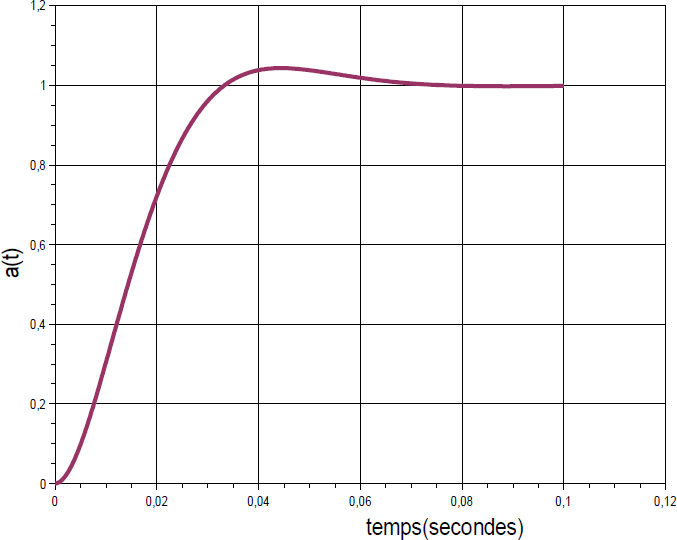
\includegraphics[width=.8\textwidth]{png/image15.png}
\end{center}

\section{Etude de l'asservissement global}
La boucle d'asservissement en décélération est donnée ci-après :

\begin{center}
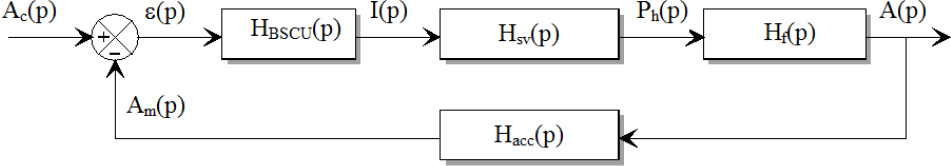
\includegraphics[width=.8\textwidth]{png/image16.png}
\end{center}

avec : 
$$
H_{sv}=\dfrac{K_{sv}}{\left(1+T_{sv} \right)^2}
$$
$$
H_{acc}=\dfrac{K_{acc}}{1+\dfrac{2\xi_a }{\omega_a}p+\dfrac{p^2}{\omega_a^2}}
$$
$$
H_f(p)=K_f
$$

$$
H_{BSCU}=K_c
$$
\paragraph{}
\textit{Exprimer sous forme canonique la fonction de transfert en boucle ouverte. En déduire
l’ordre, la classe et le gain de la $FTBO(p)$.}

\paragraph{}
\textit{Exprimer l'écart $\varepsilon(p)$ en fonction de $a_c(p)$ et de la $FTBO(p)$.}

\paragraph{}
\textit{En déduire l'écart en régime permanent à une entrée de type échelon d'accélération
$a_c (t)=a_cu (t)$. Que peut on dire de la performance de précision pour ce correcteur ?}

\paragraph{}
\textit{On utilise un correcteur (correcteur PI) plus évolué de fonction de transfert
$H_{BSCU}=K_i\dfrac{1+T_i p}{p}$, déterminer à nouveau l'écart en régime permanent et conclure sur ce choix de correcteur.}



\begin{center}
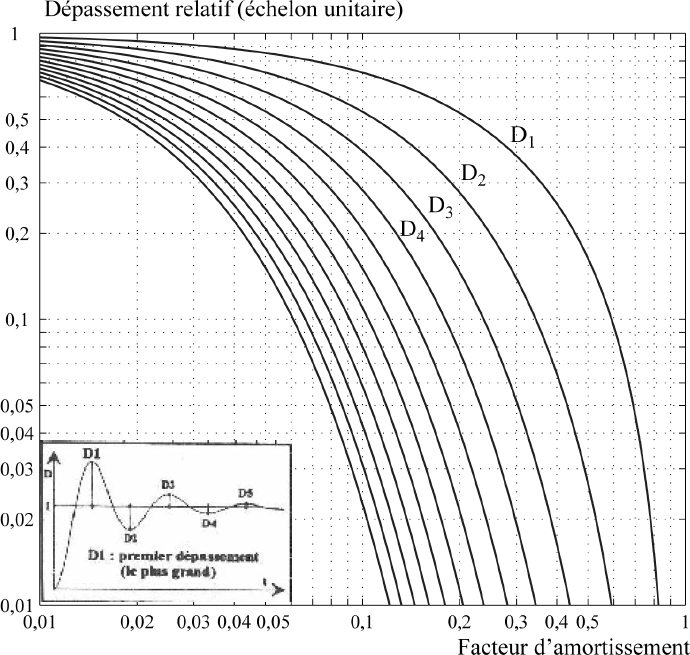
\includegraphics[width=.8\textwidth]{png/image17.png}
\end{center}

\begin{center}
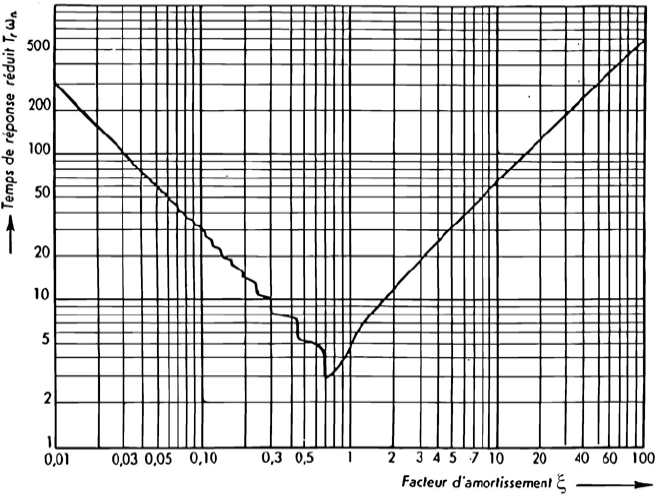
\includegraphics[width=.8\textwidth]{png/image18.png}
\end{center}

\begin{center}
\Large\textsc{-- Bon WeekEnd --}
\end{center}


\newpage{}

\section*{Documents réponse}
\begin{center}
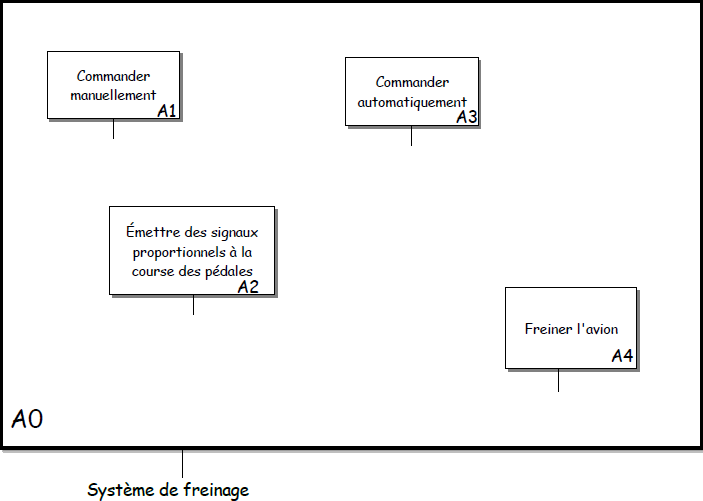
\includegraphics[width=\textwidth]{png/image19.png}
\end{center}

\begin{center}
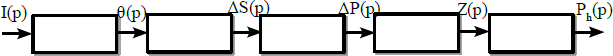
\includegraphics[width=\textwidth]{png/image20.png}
\end{center}

\end{document}

